

\documentclass{beamer}

\mode<presentation> {

% The Beamer class comes with a number of default slide themes
% which change the colors and layouts of slides. Below this is a list
% of all the themes, uncomment each in turn to see what they look like.


\usetheme{Boadilla}



\setbeamertemplate{footline}  


}
\setbeamersize{text margin left=1cm, }
\setbeamertemplate{frametitle}[default][center]
\usepackage{graphicx} 
\usepackage{booktabs} 

	\usepackage{changepage}


\usepackage{cite}
\usepackage{setspace}
\usepackage{color}
\usepackage[normalem]{ulem}
\newtheorem{hyp}{Hypothesis}


\usepackage{epsfig}
\usepackage{amsmath}
\usepackage{amssymb}
\usepackage{multicol}
\usepackage{amsmath, amsthm, amssymb}


\usepackage{graphicx}
\usepackage{tikz}
\usetikzlibrary{shapes,arrows}
\usepackage{tikz}
\usepackage{amsmath, amsthm, amssymb}
%----------------------------------------------------------------------------------------
%	TITLE PAGE
%----------------------------------------------------------------------------------------



\begin{document}
	

  

\begin{frame}
	\frametitle{Social Network Analysis}


\end{frame}




\begin{frame}
	\frametitle{Basic concepts}
	\begin{itemize}[<+->]
		\item \alert{Node} (vertex): each of the units in the network
		\item \alert{Edge} (tie): connection between nodes
		\begin{itemize}
			\item Undirected: symmetric connection, represented by lines
			\item Directed: imply direction, represented by arrows
		\end{itemize}
		\item A \alert{network} consists of a set of nodes and edges
	\end{itemize}
\end{frame}

\begin{frame}
	\frametitle{Basic concepts}
	A few examples:
	\begin{itemize}[<+->]
		\item Classroom: students / friendships
		\item Twitter: users / retweets
		\item Academic literature: papers / citations
		\item Internet: websites / hyperlinks
		\item Trade: countries / trade flows
		\item Biology: neurons / connections
	\end{itemize}
	
\end{frame}

\begin{frame}
	\frametitle{Basic concepts}
	
	\begin{columns}[T]
		\begin{column}{0.5\textwidth}
			\alert{Network Visualization}\\
			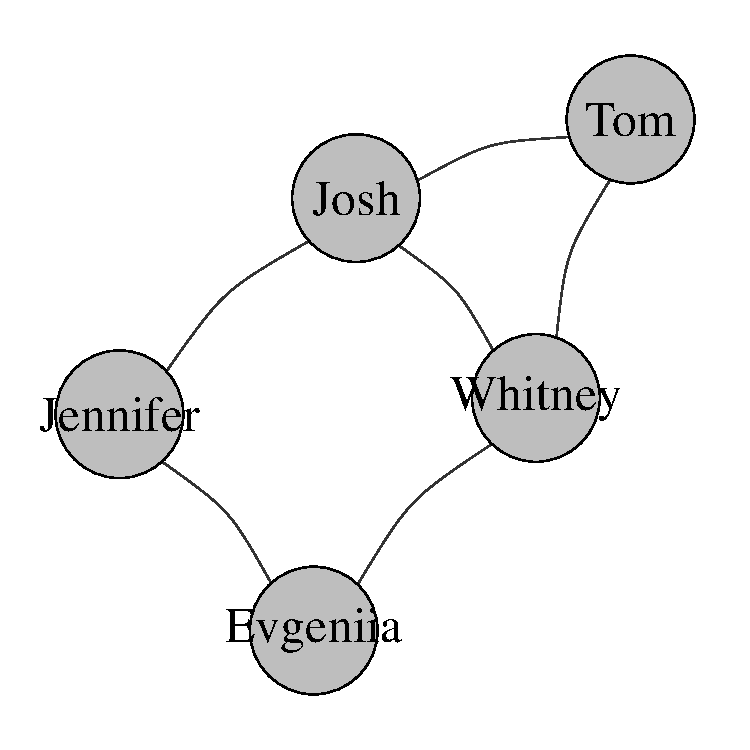
\includegraphics[width=1\textwidth]{figures/network-example.pdf}
		\end{column}
		\begin{column}{0.5\textwidth}
			\alert{Adjacency Matrix}\\
			\vspace{.50cm}
			\begin{tabular}{l|rrrrr}
				& J & J & E & W & T \\ \hline
				J & 0 & 1 & 1 & 0 & 0 \\ 
				J & 1 & 0 & 0 & 1 & 1 \\ 
				E & 1 & 0 & 0 & 1 & 0 \\ 
				W & 0 & 1 & 1 & 0 & 1 \\ 
				T & 0 & 1 & 0 & 1 & 0 \\ 
			\end{tabular}
		\end{column}
	\end{columns}
\end{frame}

\begin{frame}
	\frametitle{Basic concepts}
	
	\begin{columns}[T]
		\begin{column}{0.5\textwidth}
			\alert{Network Visualization}\\
			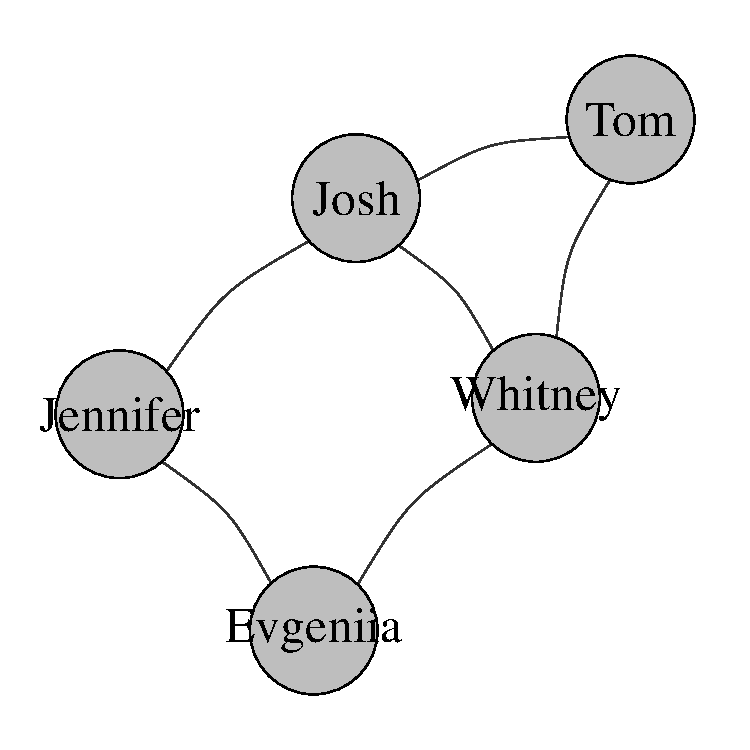
\includegraphics[width=1\textwidth]{figures/network-example.pdf}
		\end{column}
		\begin{column}{0.5\textwidth}
			\alert{Edgelist}\\
			\vspace{.50cm}
			\begin{tabular}{rll}
				\hline
				& Node1 & Node2 \\ 
				\hline
				1 & Jennifer & Josh \\ 
				2 & Jennifer & Evgeniia \\ 
				3 & Josh & Whitney \\ 
				4 & Josh & Tom \\ 
				5 & Whitney & Tom \\ 
				6 & Evgeniia & Whitney \\ 
				\hline
			\end{tabular}
		\end{column}
	\end{columns}
\end{frame}



\begin{frame}
	\frametitle{Latent structure of social networks}
	
	\includegraphics<1>[width=\textwidth]{figures/mynetwork1.png}
	\includegraphics<2>[width=\textwidth]{figures/mynetwork2.png}

	
\end{frame}


\begin{frame}
	\frametitle{The dreaded \textit{hairball}}
	
	\includegraphics<1>[width=.75\textwidth]{figures/04-community-network-v3-small.png}
	
\end{frame}

\begin{frame}
	\frametitle{Discovery in large-scale networks}
	
	How to understand the structure of large-scale networks?
	
	\begin{itemize}[<+->]
		\item Latent \alert{communities} or clusters
		\begin{itemize}
			\item \textbf{Community detection algorithms}
			\item Finding groups of nodes that \alert{densely connected internally}, more so than to the rest of the networks
			\item Overlap with shared visible or latent similarities (homophily)
			\item Also \alert{hierarchy}: core-periphery detection
		\end{itemize}
		\vspace{.20cm}
		\item Locating nodes on \alert{latent spaces}
		\begin{itemize}
			\item \textbf{Latent space models of networks}
			\item Proximity on latent space (ideology) predicts existence of edges
			\item Inference about latent positions based on multidimensional scaling of the adjacency matrix
		\end{itemize}
	\end{itemize}
	
	
\end{frame}


\begin{frame}
	\frametitle{Community detection}
	\begin{columns}
		\column{.55\linewidth}
		\alert{Community structure:}
		\begin{itemize}
			\item Network nodes often cluster into tightly-knit groups with a {\color{red}{high density of within-group edges}} and a {\color{blue}{lower density of between-group edges}}
			\item \textbf{Modularity score}: measures clustering of nodes compared to random network of same size
			\item Many different \alert{community detection algorithms} based on different assumptions
		\end{itemize}
		
		\column{.48\linewidth}
		\centering
		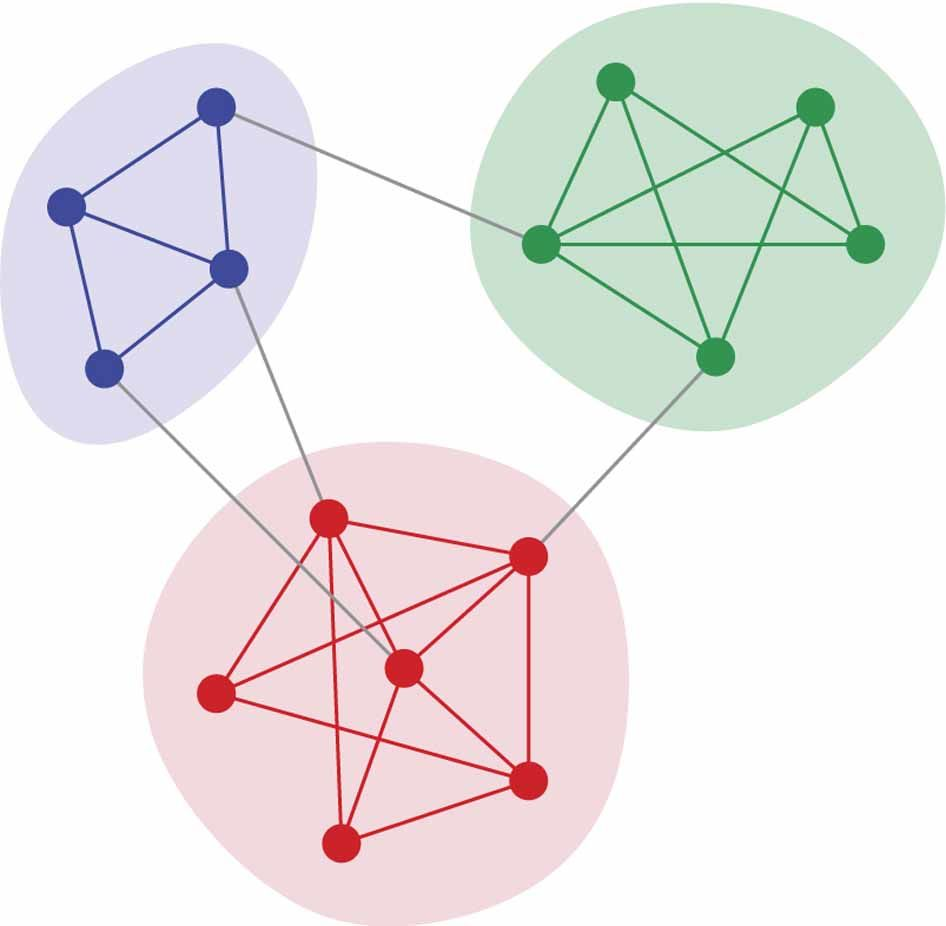
\includegraphics[width=1\textwidth]{figures/modularity.jpg}\\
		\textbf{Source}: Newman (2012)
	\end{columns}
\end{frame}


\begin{frame}
	\frametitle{Network hierarchy}
	
	\begin{itemize}[<+->]
		\item \textbf{Intuition}
		\begin{itemize}
			\item Large-scale networks have hierarchical properties
		\end{itemize}
		\item \textbf{Network core:}
		\begin{enumerate}
			\item \textit{Centrality}: high relative importance in network 
			\item \textit{Connectivity}: many possible distinct paths between individuals
			\item[] (not captured by simple topological measures)
		\end{enumerate}
		\item \textbf{k-core decomposition}
		\begin{itemize}
			\item Algorithm to partition a network in nested shells of connectivity
			\item The \textit{k}-core of a graph is the maximal subgraph in which every node has at least degree \textit{k} 
			\item Many applications; scales well to large networks: $\mathcal{O}(n+e)$
		\end{itemize}
	\end{itemize}
\end{frame}

\begin{frame}
	\frametitle{k-core decomposition}
	
	\centering\includegraphics<1>[width=.7\linewidth]{figures/kcore1.pdf}
	\centering\includegraphics<2>[width=.7\linewidth]{figures/kcore2.pdf}\\
	Source: Alvarez-Hamelin et al, 2005
\end{frame}

{ 
	\begin{frame}[plain]
		\begin{tikzpicture}[remember picture,overlay]
		\node[at=(current page.center)] {
			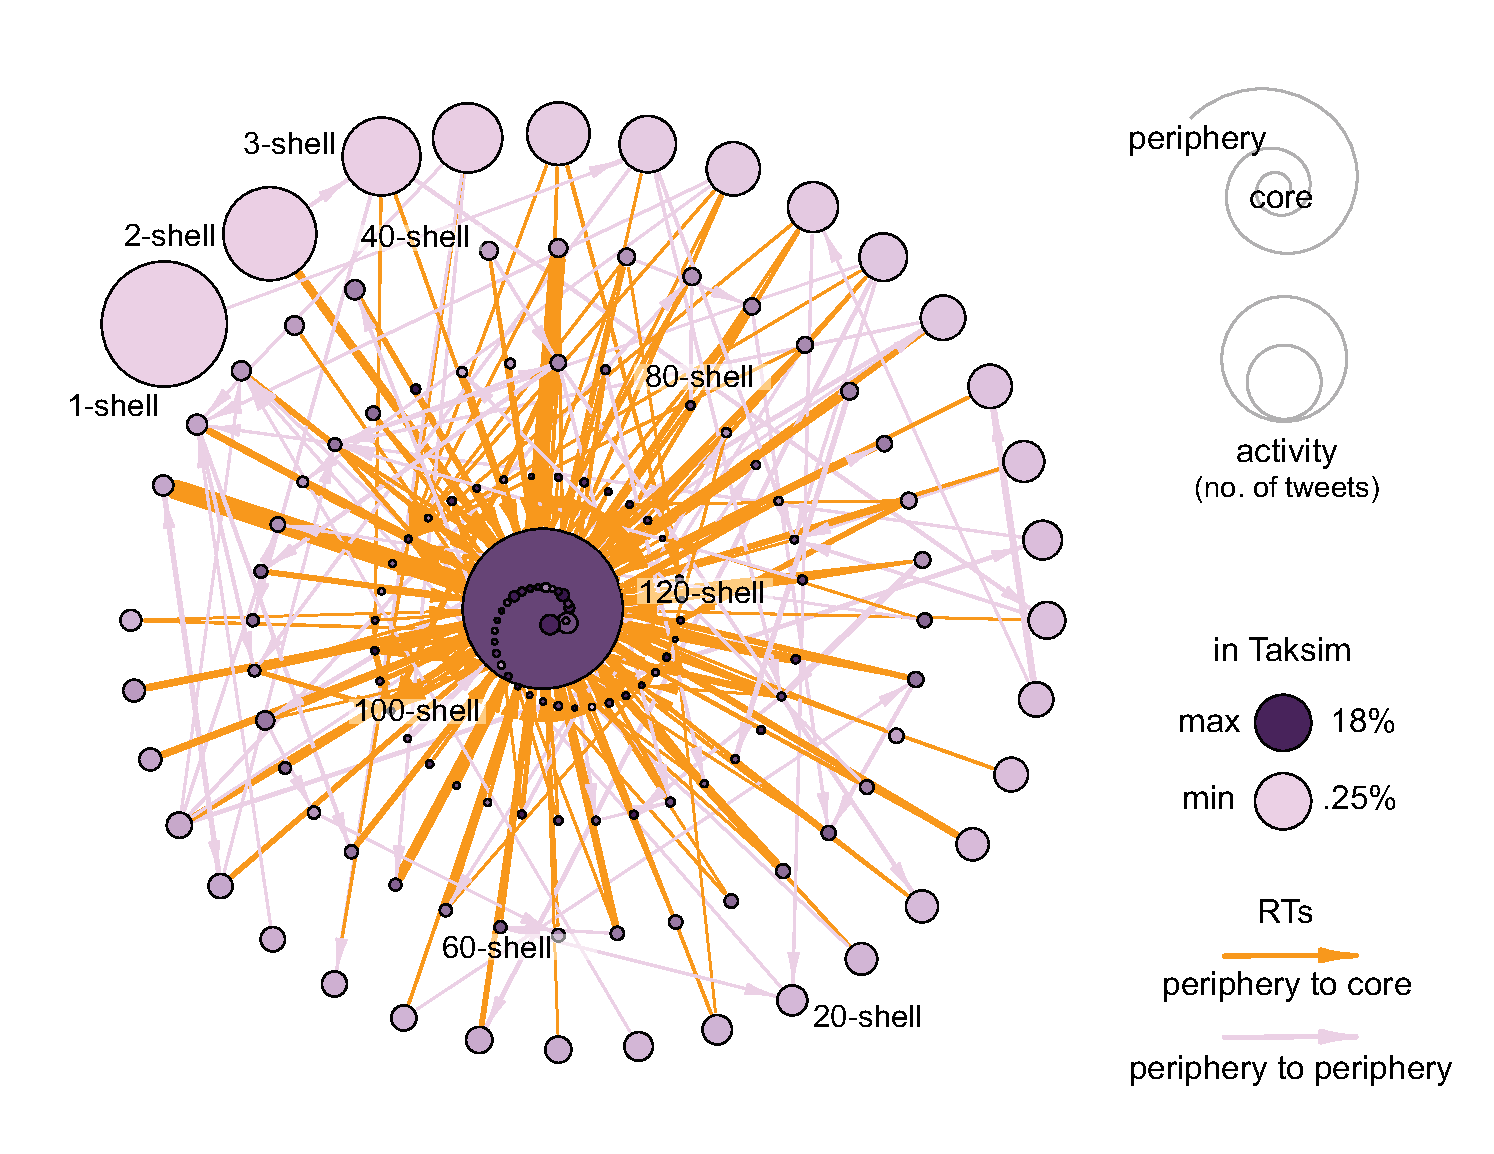
\includegraphics[height=\paperheight]{figures/fig3.eps}
		};
		\node[anchor=north west] [at=(current page.north west)]{
			\alert{\Large{k-core decomposition of \#OccupyGezi network}}
		};
		\end{tikzpicture}
		
	\end{frame}
}

{ 
	\begin{frame}[plain]
		\begin{tikzpicture}[remember picture,overlay]
		\node[yshift=1cm] (picture) [at=(current page.center)] {
			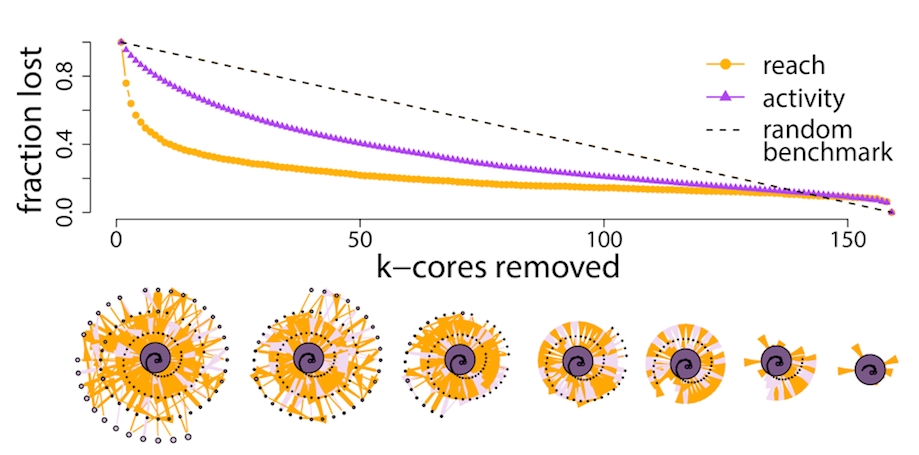
\includegraphics[width=\paperwidth]{figures/simulation-turkey.png}
		};
		\node[anchor=north west] [at=(current page.north west)]{
			\alert{\Large{Relative importance of core and periphery}}
		};
		\node[anchor=north west, xshift=1cm] (reach) [at=(picture.south west)]{
			\alert{reach}: aggregate size of participants' audience
		};
		\node[anchor=north west, xshift=0cm] [at=(reach.south west)]{
			\alert{activity}: total number of protest messages published (not only RTs)
		};
		\end{tikzpicture}
		
	\end{frame}
}






\end{document} 